\section{Лист 1}
    \begin{prob}
        Вычислите число неубываюпих путей на целочистенной репетке $\mathbb{Z}^{2}$ (то есть таких, что за один шаг происходит сдвиг на единицу либо вправо, либо вверх), ведунцих из точки $(0,0)$ в точку $(n, n)$, и не пересеканопих диагональ (то есть, проходяпих только через такие точки $(i, j)$, для которых $j \leq i$). Затем почитать в Википедии про числа Каталана.
    \end{prob}
    \begin{proof}
        Всего путей из $(0,0)$ в $(n,n)$ ровно ${{2n}\choose{n}}$, так как нужно сделать всего $2n$ шагов, среди которых $n$ в одном направлении и $n$ в другом. Посчитаем пути выше диагонали, замтим что можно построить биекцию между этими путями и путями из $(-1, 1)$ (или $(1, -1)$) в $(n,n)$. Заметим что таких путей ровно ${{2n}\choose{n-1}}$, тогда путей ниже диагонали ${{2n}\choose{n}} - {{2n}\choose{n-1}} = \frac{1}{n+1} {{2n}\choose{n}}$
    \end{proof}
\vskip 0.6in


    \begin{prob}
        Имеется код длины $n$, состояцций из цифр от $0$ до $9$. Найдите вероятность того, что цифры в коде расположены в неубывающем порядке.
    \end{prob}
    \begin{proof}
        Заметим, что если последовательность неубывающая, то она имеет вид $0, \ldots, 0, 1 ,\ldots, 9$ (какие-то цифры могут отсутствовать), то есть это количество способов расставить $9$ перегородок на $(n-1) + 9 = n+8$ позиций, то есть ${{n+8}\choose{9}}$
    \end{proof}
\vskip 0.6in


    \begin{prob}
        Из мешка, в котором лежат все кости набора домино (их $28$ штук, соответствующих неупорядоченным парам чисел от $0$ до $6$), извлекают две костяшки. Найдите вероятность того, что их можно приложить друг к другу по правилам игры в домино.
    \end{prob}
    \begin{proof}
        Всего пар костяшек $\frac{28 \cdot 27}{2}$, посчитаем число тех, которые можно сложить вместе. Каждая костяшка с 2 одинаковыми значениями может быть в паре с $6$ другими, а с $2$ разными значениями --  в паре с $12$, откуда
        \begin{gather*}
            \frac{\frac{7 \cdot 6 + (28-7) \cdot 12}{2}}{\frac{28 \cdot 27}{2}}
            = \frac{7 \cdot 6 + (28 - 7) \cdot 12}{28 \cdot 27}
            = \frac{7 \cdot 2 + 21 \cdot 4}{28 \cdot 9}
            = \frac{7 \cdot 14}{28 \cdot 9}
            = \frac{7}{18}
        \end{gather*}
    \end{proof}
\vskip 0.6in


    \begin{prob}
        На экзамене студенты по очереди вытягиванот билеты (и, естественно, не возвращают их на место). Всего имеется $n$ билетов, из которых $k$ - простые, и $m \leq n$ студентов. Чему равна вероятность того, что первый студент вытянет простой билет? А последний? Меняется ли вероятность вытянуть простой билет в зависимости от того, каким номером студент тянет билет?
    \end{prob}
    \begin{proof}
        Добавим еще $n-m$ студентов, чтобы сткдентов было столько же, сколько и билетов, далее пронумеруем студентов от 1 до $n$ в соответствии с очередью. Также пронумеруем билеты от 1 до $n$, тогда вероятностное пространство:
        \begin{gather*}
            \Omega=\left\{\left(i_{1}, i_{2}, \ldots i_{n}\right) \mid 1 \leqslant i_{a} \leqslant n,\ i_{b} \neq i_{c},\ b \neq c\right\}
        \end{gather*}
        Элементарным событием является перестановка $\left(i_{1}, i_{2} \ldots i_{n}\right)$, где $i_j$ -- номер билета у студента с номером $j$.
        \vskip 0.1in
        $A_{i\: 1}$ -- студент под номером $i$ получил билет номер $1$, равновероятно событию $A_{i\ 2}$, так как между множествами перестановок, в которых $i$ студент получил билет номер $1$ и $2$, существует биекция. Аналогичном, события $\left\{A_{i\: 1}, A_{i\: 2}, \ldots A_{i\: n}\right\}$ равновероятны.
        \vskip 0.1in
        Событие $B_{j}$ студент $j$ вытянул простой билет, $\mathcal{P}(B_{j})=\frac{k}{n}$ для любого $j$, откуда вероятность вытягивания простого билета у всех студентов равна $\frac{k}{n}$.
    \end{proof}
\vskip 0.6in


    \begin{prob}
        Пассажиры заходят в самолет и рассаживаются случайным образом, не обрашая внимания на свои билеты. С какой вероятностью ни один пассажир не сядет на свое место?
    \end{prob}
    \begin{proof}
        То есть мы хотим рассмотреть отношение числа перестановки из $n$ элементов без неподвижной точки к общему числу перестановок, для этого мы вычтем из общего числа перестановок $n!$, число перестановок с $k$ неподвижными точками ${{n}\choose{k}} (n-k)!$
        \begin{gather*}
            \mathcal{P} = \frac{|A|}{|\Omega|}
            = \frac{n! - {{n}\choose{1}} (n-1)! + {{n}\choose{2}} (n-2)! - \ldots}{n!}\\
            = \frac{n! \cdot \left(1 - \frac{1}{1!} + \frac{1}{2}! - \ldots + (-1)^n \frac{1}{n!}\right)}{n!}\\
            = \frac{n! \cdot \sum\limits_{k = 0}^{n} \frac{(-1)^k}{k!}}{n!}
            = \sum\limits_{k = 0}^{n} \frac{(-1)^k}{k!}
        \end{gather*}
    \end{proof}
\vskip 0.6in


    \begin{prob}
        Профессор разбирает на семинаре $k$ задач, вызывая для каждой из них одного из $n$ присутствуюпих студентов случайным образом. Какова вероятность того, что к концу семинара каждый из студентов побывает у доски не более двух раз?
    \end{prob}
    \begin{proof}
        \begin{gather*}
            \Omega = \{(\omega_1, \ldots, \omega_k)\ |\ \omega_j = \{1, \ldots, n\} \}\\
            \Omega = \{(\omega_1, \ldots, \omega_k)\ |\ \omega_j = \{1, \ldots, n\} \text{ не более 2 повторений} \}
        \end{gather*}
        Тогда посчитаем число элементов в каждом из этих множеств, $|\Omega|$ -- каждую из $k$ задач может разобрать один из $n$ студентов
        \begin{gather*}
            |\Omega| = n^k
        \end{gather*}
        Подсчет числа искомых варинатов можно представить как способ выборать $k$ элементов из $2n$ (то есть двойной набор студенов)
        \begin{gather*}
            |A| = \frac{\# \{1, \ldots, n, \tilde{1}, \ldots, \tilde{n}\}}{(2!)^n}
            = \frac{2n \cdot (2n-1) \cdot \ldots \cdot (2n-k+1)}{(2!)^n}
            = \frac{(2n)!}{(2n-k)! 2^n}
        \end{gather*}
        Откуда
        \begin{gather*}
            \mathcal{P}(A) = \frac{|A|}{|Q|} = \frac{(2n)!}{(2n-k)! \cdot 2^n \cdot n^k}
        \end{gather*}
    \end{proof}
\vskip 0.6in


    \begin{prob}
        Приведите пример $n$ случайных событий, таких что любые $n-1$ из них независимы (в совокупности), а все они вместе - зависимы.
    \end{prob}
    \begin{proof}
        Пусть события $A_i,\ i \in [1, n-1]$ -- выпадение орла (при броске монеты), а $A_n$ -- выпало четное число орлов, тогда $\{A_1, \ldots, A_n\}$ зависимо, но любое подмножество независимо
    \end{proof}
\vskip 0.6in


    \begin{prob}
        Тест на ковид имеет чувствитетьность $50\%$ (т.е. верно диагностирует больного в $50\%$ случаев) и специфичность $70\%$ ($30\%$ здоровых людей обььявляет больными). Известно, что на данной территории ковидом болеет 1 человек из $300$. Какова вероятность того, что житель этой территории, обьявленный больным по результатам теста, действителыно болен?
    \end{prob}
    \begin{proof}
        Обозначим через ``+'' положительный результат теста и через ``-'' отрицательный, тогда
        \begin{gather*}
            P(+|\text{болен}) = 0.5\qquad
            P(+|\text{здоров}) = 0.3\\
            P(-|\text{болен}) = 1 - 0.5 = 0.5\qquad
            P(-|\text{здоров}) = 1 - 0.3 = 0.7\\
            P(\text{болен}) = \frac{1}{300}\\
            P(\text{здоров}) = \frac{299}{300}\\
        \end{gather*}
        Чтобы решить задачу, воспользуемся формулой Байеса:
        \begin{gather*}
            P(\text{болен}| +)
            = \frac{P(+|\text{болен}) P(\text{болен})}{P(+|\text{болен}) P(\text{болен}) + P(+|\text{здоров}) P(\text{здоров})}
            = \frac{\frac{1}{300} \cdot \frac{1}{2}}
            {\frac{1}{300} \cdot \frac{1}{2} + \frac{299}{300} \cdot \frac{3}{10}} = \frac{5}{2 \cdot 11 \cdot 41} \approx 0.006
        \end{gather*}  
    \end{proof}
\vskip 0.6in


    \begin{prob}
        Треугольник $A B C$ - прямоугольный равнобедренный с прямым углом $C$ и катетами, равными 1. В нём случайным образом выбирается точка $Z$. Пусть $X$ и $Y$-основания перпендикуляров из $Z$ на катеты. Обозначим буквами $P$ и $S$ соответственно периметр и площадь прямоугольника $C X Z Y$.
        \begin{itemize}
            \item[(a)] Найдите вероятность того, что $S < \frac{8}{81}$.
            \item[(b)] Найдите вероятность того, что $P < \frac{4}{3}$.
            \item[(c)] Найдите условную вероятность того, что $S < \frac{8}{81}$ при условии, что $P < \frac{4}{3}$
            \item[(d)] Найдите условную вероятность того, что $P < \frac{4}{3}$ при условии, что $S < \frac{8}{81}$.
            \item[(e)] Существуют ли такие числа $S_{0} \in (0, \frac{1}{4})$ и $P_{0} \in (0, 2)$, что события $\left\{ S < S_{0} \right\}$ и $\left\{ P < P_{0} \right\}$ будут независимы?
        \end{itemize}
    \end{prob}
    \begin{proof}
        Заметим, что все это вероятности являются отношением площади ГМТ подходящих под условие точек к площади всего трегуольника. Заранее посчитаем площади зеленой и синих частей
        \begin{figure}[h]
            \center{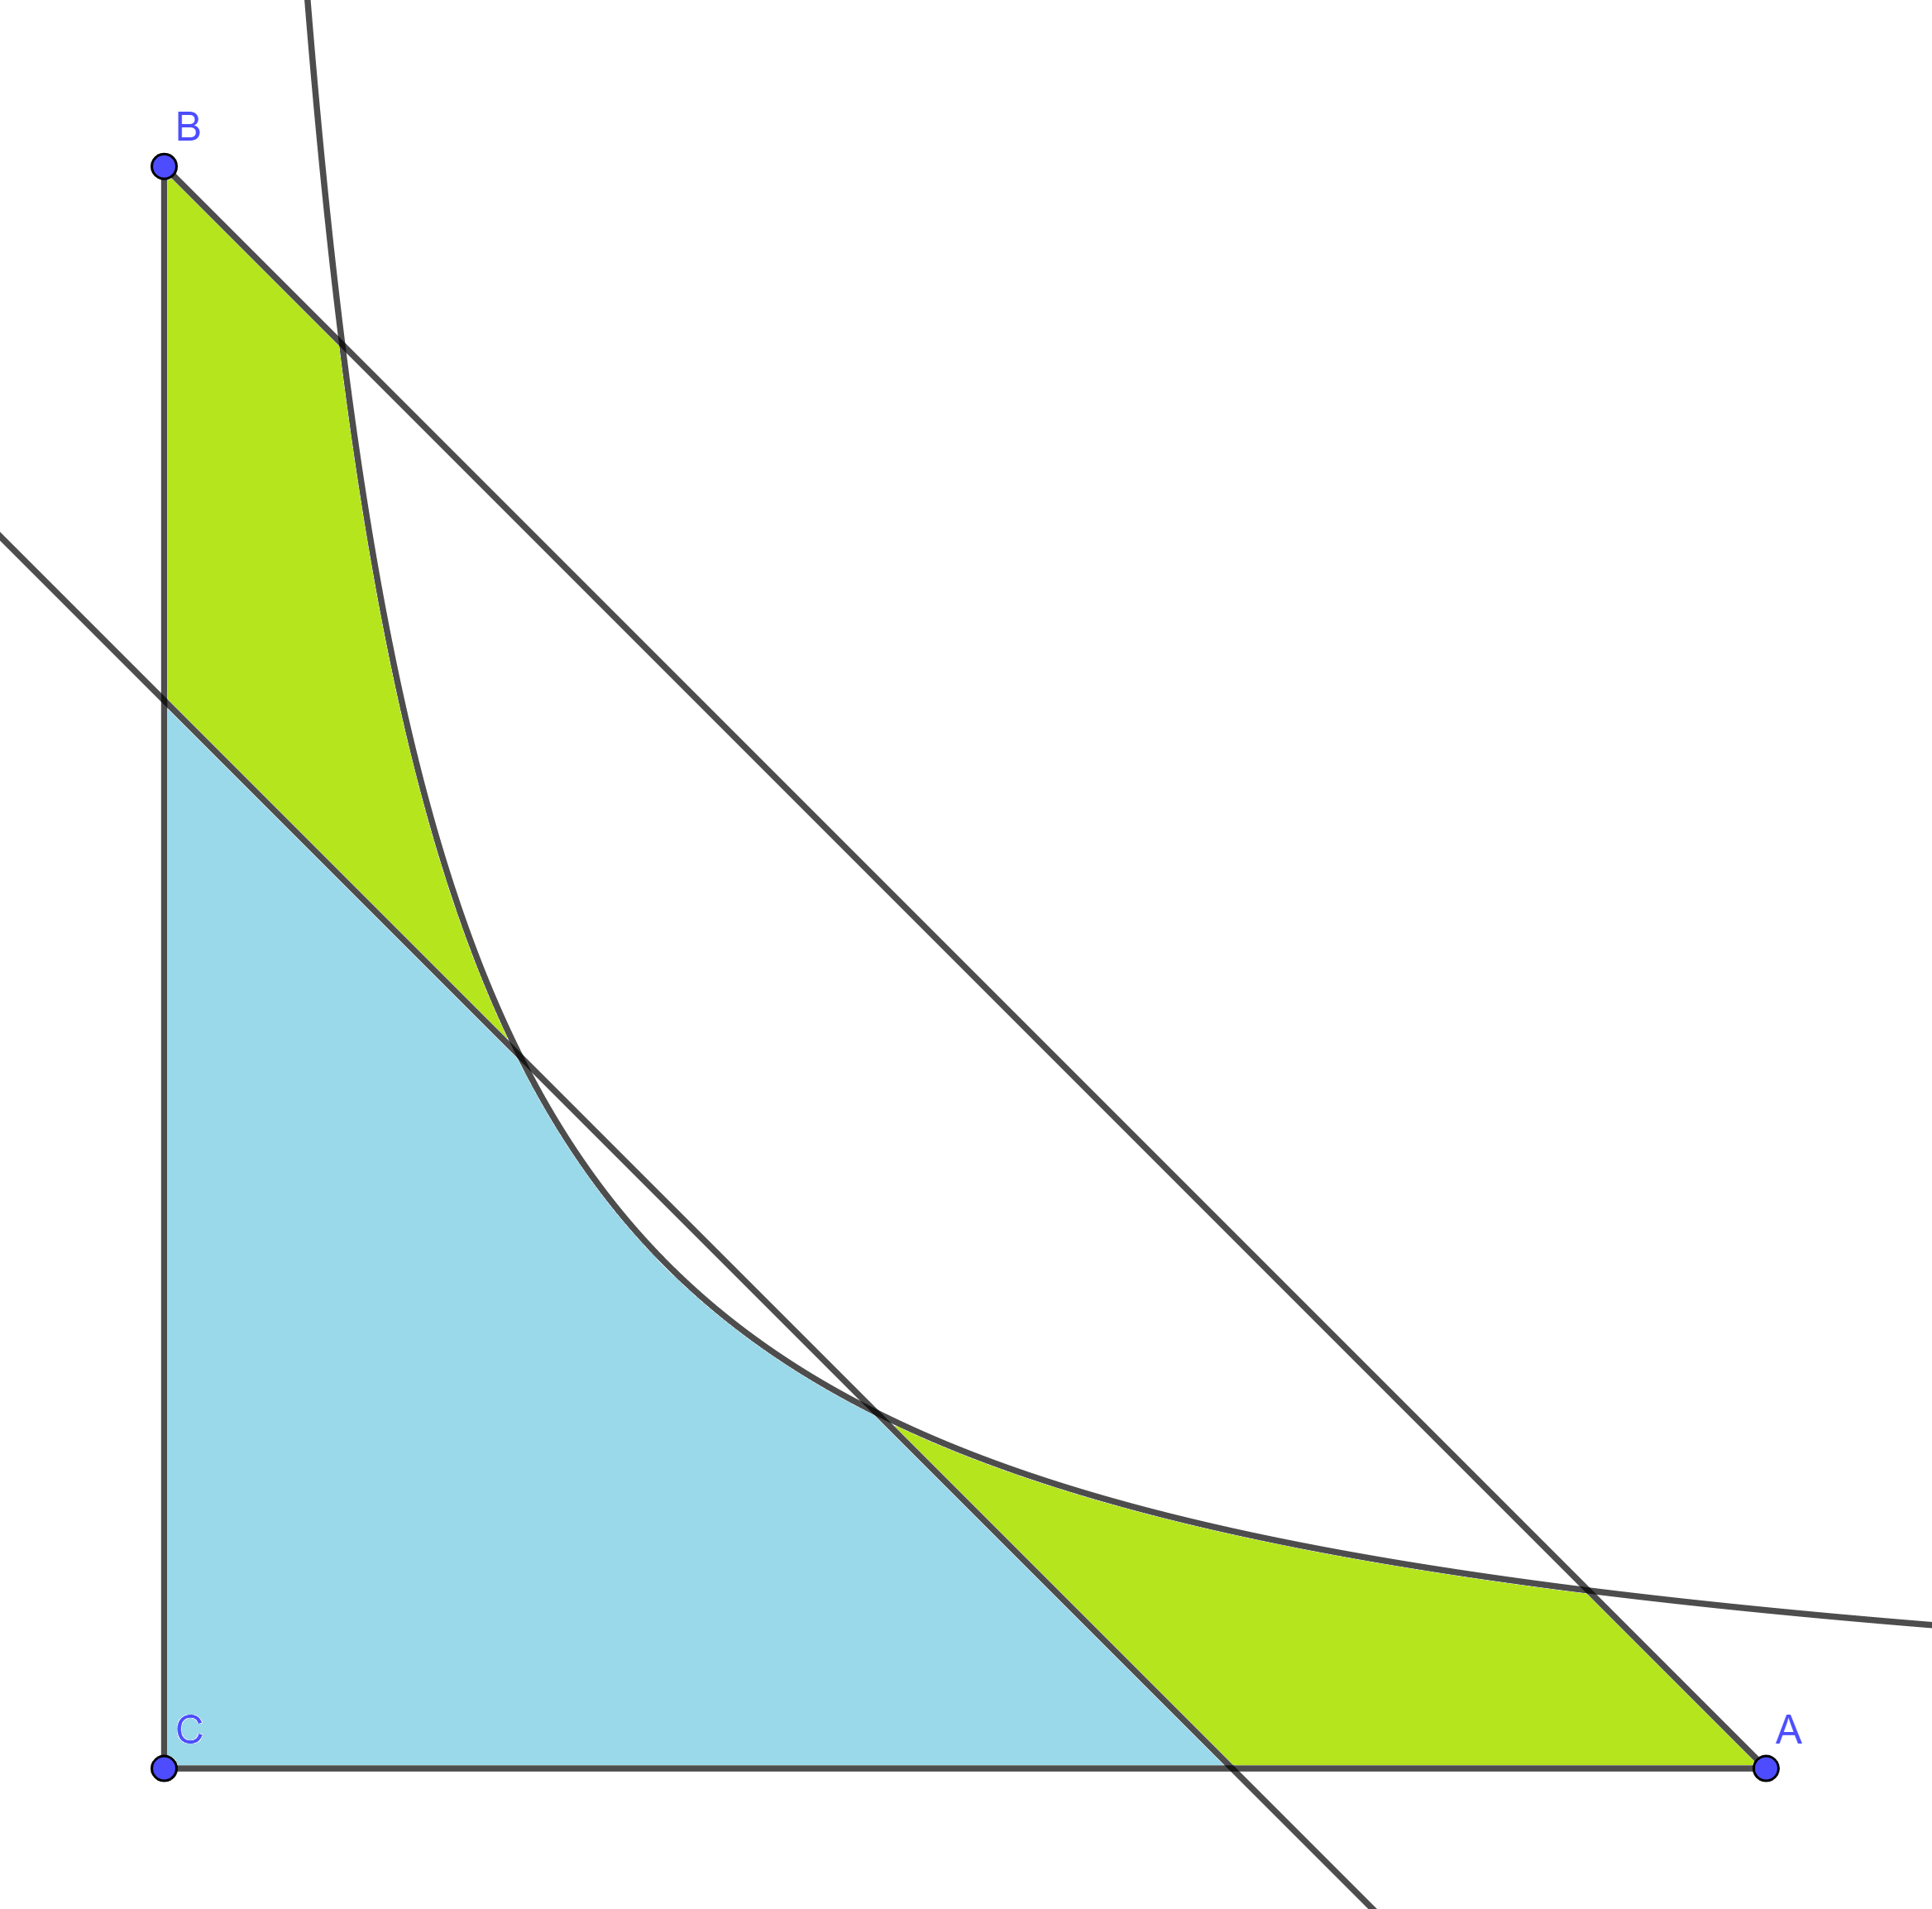
\includegraphics[width=0.8\linewidth]{IMG_1}}
        \end{figure}
        \begin{gather*}
            \begin{cases}
                y + x - \frac{2}{3} = 0\\
                y - \frac{8}{81 x} = 0
            \end{cases}\\
            \frac{8}{81 x} = -x + \frac{2}{3}\\
            81x^2 - 54x + 8 = 0\\
            x_1 = \frac{4}{9}\qquad y_1 = \frac{2}{9}\\
            x_2 = \frac{2}{9}\qquad y_2 = \frac{4}{9}\\
            \int\limits_{\frac{2}{9}}^{\frac{4}{9}} \frac{8}{81x} dx
            = \frac{8}{81} \ln x \bigg|_{\frac{2}{9}}^{\frac{4}{9}}
            = \frac{8}{81} (\ln \frac{4}{9} - \ln \frac{2}{9})
            = \frac{8}{81}\ln 2\\
            \frac{4}{27} + \frac{8}{81} \ln 2 
        \end{gather*}
        И
        \begin{gather*}
            \int\limits_{\frac{4}{9}}^{\frac{8}{9}} \frac{8}{81 x} dx
            = \frac{8}{81} \ln x \bigg|_{\frac{4}{9}}^{\frac{8}{9}}
            = \frac{8}{81} \left(\ln \frac{8}{9} - \ln \frac{4}{9}\right)
            = \frac{8}{81} \ln 2\\
            \frac{8}{81} \ln 2 - \frac{2}{81} = \frac{2}{81} (4\ln 2 - 1)
        \end{gather*}
        \begin{itemize}
            \item[(a)] Заметим что подходящие точки ограничены сторонами треугольника и кривой $y = \frac{8}{81 x}$, то есть ответ является отношением площади этой части к площади всего треугольника, то есть
            \begin{gather*}
                \frac{2 \cdot \frac{2}{81}(4 \ln 2 - 1) + \left(\frac{4}{27} + \frac{8}{81} \ln 2\right)}{\frac{1 \cdot 1}{2}}
                = \frac{\frac{8}{81}\left(3 \ln 2 + 1\right)}{\frac{1}{2}}
                = \frac{16}{81}\left(3 \ln 2 + 1\right)
                \approx 0.6
            \end{gather*}
            \item[(b)] Заметим что $P = CX + XZ + ZY + ZY = 2(CX + CY) < \frac{4}{3}$, тогда подходящие точки ограничены сторонами треугольника и прямой $y + x - \frac{2}{3} = 0$  вероятность равна отношению этой части к площади всего треугольника
            \begin{gather*}
                \frac{\frac{\frac{2}{3} \cdot \frac{2}{3}}{2}}{\frac{1 \cdot 1}{2}}
                = \frac{4}{9}
                \approx 0.44
            \end{gather*}
            \item[(c)] Вероятность равна отношению площади зеленой части к площади под прямой $y + x - \frac{2}{3} = 0$, ограниченной сторонами треугольника
            \begin{gather*}
                \frac{\frac{4}{27} + \frac{8}{81} \ln 2}{\frac{\frac{2}{3} \cdot \frac{2}{3}}{2}}
                = \frac{2}{9}\left(3 + 2 \ln 2\right)
                \approx 0.97
            \end{gather*}
            \item[(d)] Вероятность равна отношению площади зеленой части к площади под $y = \frac{8}{81 x}$, ограниченной сторонами треугольника
            \begin{gather*}
                \frac{\frac{4}{27} + \frac{8}{81} \ln 2}{\frac{4}{27} + \frac{8}{81} \ln 2 + 2 \cdot \frac{2}{81} (4\ln 2 - 1)}
                = \frac{\frac{4}{27} + \frac{8}{81} \ln 2}{\frac{8}{81}(3 \ln 2 + 1)}
                = \frac{3 + 2 \ln 2}{6 \ln 2 + 2}
                \approx 0.71
            \end{gather*}
            \item[(e)] Независимость событий говорит о том, что $P(A \cap B) = P(A) \cdot P(B)$, то есть в нашем случае это значит, что вероятность того, что выбранная точка $Z$ будет соответствовать сразу всем условиям, равна произведению вероятности того, что она будет иметь периметр $P_0$ и вероятности того, что площадь $S_0$. Тогда мы можем записать формулу $P(A \cap B) = P(A) \cdot P(B)$ через площади, получив условие на $P_0, S_0$.
            \begin{gather*}
                \frac{1 \cdot 1}{2}
                \cdot \left(
                    \int\limits
                    _{\frac{P_0 - \sqrt{P_0^2 - 8S_0}}{2}}
                    ^{\frac{P_0 + \sqrt{P_0^2 - 8S_0}}{2}}
                    S_0 \frac{1}{x} dx
                    + \frac{P_0 - \sqrt{P_0^2 - 8S_0}}{2} \cdot \frac{P_0}{2}
                \right)
                = \frac{P_0^2}{8}
                \cdot \left(
                    \int\limits
                    _{\frac{1 - \sqrt{1 - 4S_0}}{2}}
                    ^{\frac{1 + \sqrt{1 - 4S_0}}{2}}
                    S_0 \frac{1}{x} dx
                    + \frac{1 - \sqrt{1 - 4S_0}}{2} \cdot 1
                \right)\\
                4
                \cdot \left(
                    \int\limits
                    _{\frac{P_0 - \sqrt{P_0^2 - 8S_0}}{2}}
                    ^{\frac{P_0 + \sqrt{P_0^2 - 8S_0}}{2}}
                    S_0 \frac{1}{x} dx
                    + \frac{P_0 - \sqrt{P_0^2 - 8S_0}}{2} \cdot \frac{P_0}{2}
                \right)
                = P_0^2
                \cdot \left(
                    \int\limits
                    _{\frac{1 - \sqrt{1 - 4S_0}}{2}}
                    ^{\frac{1 + \sqrt{1 - 4S_0}}{2}}
                    S_0 \frac{1}{x} dx
                    + \frac{1 - \sqrt{1 - 4S_0}}{2}
                \right)\\
                8\int\limits
                _{\frac{P_0 - \sqrt{P_0^2 - 8S_0}}{2}}
                ^{\frac{P_0 + \sqrt{P_0^2 - 8S_0}}{2}}
                S_0 \frac{1}{x} dx
                + 2 \left(P_0^2 - P_0 \sqrt{P_0^2 - 8S_0}\right)
                = 2 P_0^2
                \int\limits
                _{\frac{1 - \sqrt{1 - 4S_0}}{2}}
                ^{\frac{1 + \sqrt{1 - 4S_0}}{2}}
                S_0 \frac{1}{x} dx
                + P_0^2 (1 - \sqrt{1 - 4S_0})\\
                8\int\limits
                _{\frac{P_0 - \sqrt{P_0^2 - 8S_0}}{2}}
                ^{\frac{P_0 + \sqrt{P_0^2 - 8S_0}}{2}}
                S_0 \frac{1}{x} dx
                - 2 P_0^2
                \int\limits
                _{\frac{1 - \sqrt{1 - 4S_0}}{2}}
                ^{\frac{1 + \sqrt{1 - 4S_0}}{2}}
                S_0 \frac{1}{x} dx
                = P_0^2 \left(2\sqrt{1 - 8\frac{S_0}{P_0^2}} - \sqrt{1 - 4S_0} -1\right)\\
            \end{gather*}
        \end{itemize}
    \end{proof}
\vskip 0.6in


    \begin{prob}
        Вася и Петя ездят в школу на автобусе. Вася приходит на автобуснуго остановку в момент времени, равномерно распределённый на отрезке между $8:00$ и $8:17$, и садится в первый подопедииии автобус; если же в $8:17$ Вася всё ещё не уехал, то он бежит в школу бегом. Его одноклассник Петя поступает ровно таким же образом. Автобусы подьезжанот к остановке каждые $5$ минут (время прибытия первого из них равномерно распределено на отрезке от $8:00$ до $8:05$). Kaкова вероятность того, что Вася и Петя поедут в пколу на одном и том же автобусе, если времена появления на остановке Васи, Пети и первого автобуса независимы?
    \end{prob}

    \begin{proof}
        Вероятностное пространство имеет вид $\Omega = \{\omega_n\ |\ n \in [0,17]\}$, события $\omega_n$ = прийти на остановку в $8:n$, $A_1 := (\text{будет 3 автобуса})$, то есть первый автобус приехал в $\left(2, 5\right]), \mathcal{P}(A_1) = \frac{3}{5}$, $A_2 := (\text{приедет 4 автобуса})$, то есть первый в $\left[0, 2\right]), \mathcal{P}(A_2) = \frac{2}{5}$. $\omega_{P} = t_1$ -- Петя пришел в $t_1$, $\omega_{V} = t_2$ -- Вася пришел в $t_2$. Петя и Вася будут в одном автобусе только в том случае, если они придут в один временной промежуток, так как события $\{A_1, \omega_{P}, \omega_{V}\}$ независимы, то
        \begin{gather*}
            \frac{x_1}{17} \cdot \frac{x_1}{17} + 2 \cdot \frac{5}{17} \cdot \frac{5}{17}
            = \frac{9 + 2 \cdot 5^4}{17^2 \cdot 5^2}
            = \frac{1259}{7225}
        \end{gather*}
        Аналогично $\{A_2, \omega_{P}, \omega_{V}\}$ независимы
        \begin{gather*}
            \frac{x_2}{17} \cdot \frac{x_2}{17} + 3 \cdot \frac{5}{17} \cdot \frac{5}{17}
            = \frac{2^2 + 3 \cdot 5^4}{17^2 \cdot 5^2}
            = \frac{1879}{7225}
        \end{gather*}
        Тогда итоговая вероятность
        \begin{gather*}
            \frac{1259}{7225} + \frac{1879}{7225}
            = \frac{3138}{7225}
            \approx 0.43
        \end{gather*}
    \end{proof}
\vskip 0.6in


    \begin{prob}
        На гранях двух кубиков расставлены натуральные числа $k_{1}, \ldots, k_{6}$. $l_{1}, \ldots, l_{6}$ cooтветственно, причём неверно, что $\left\{k_{1}, \ldots, k_{6}\right\}=\left\{l_{1}, \ldots, l_{6}\right\} = \{1, \ldots, 6\}$. Можно ли подобрать числа $k_{i}, l_{j}$ так, что для любого $s=2, \ldots, 12$ вероятность того, что при броске этих кубиков выпадет сумма очков, равная $s$, совпадает с той же вероятностью для «классических» кубиков (с цифрами от $1$ до $6$ на гранях)?
    \end{prob}
    \begin{proof}
        Рассмотрим кости с числами $\{1, 2_1, 2_2, 3_1, 3_2, 4\}$ (в данном случае индекс лишь обозначает несколько одинаковых значений) и $\{1, 3, 4, 5, 6, 8\}$, заметим, что вероятность выпадения каждой из сумм совпадает с вероятностью выпадения на классических кубиках. В следующей таблицы приведены все возможные исходы, причем они все равновероятны
        \begin{center}
            \begin{tabular}{ |c|cccccc| } 
                \hline
                2 & $\{1, 1\}$ &&&&& \\ 
                \hline
                3 & $\{2_1, 1\}$ & $\{2_2, 1\}$ &&&& \\ 
                \hline
                4 & $\{3_1, 1\}$ & $\{3_2, 1\}$ & $\{1, 3\}$ &&& \\ 
                \hline
                5 & $\{1, 4\}$ & $\{2_1, 3\}$ & $\{2_2, 3\}$ & $\{4, 1\}$ && \\ 
                \hline
                6 & $\{1, 5\}$ & $\{2_1, 4\}$ & $\{2_2, 4\}$ & $\{3_1, 3\}$ & $\{3_2, 3\}$ & \\ 
                \hline
                7 & $\{1, 6\}$ & $\{2_1, 5\}$ & $\{2_2, 5\}$ & $\{3_1, 4\}$ & $\{3_2, 4\}$ & $\{4, 3\}$ \\ 
                \hline
                8 & $\{2_1, 6\}$ & $\{2_2, 6\}$ & $\{3_1, 5\}$ & $\{3_2, 5\}$ & $\{4, 4\}$ & \\ 
                \hline
                9 & $\{1, 8\}$ & $\{3_1, 6\}$ & $\{3_2, 6\}$ & $\{4, 5\}$ && \\ 
                \hline
                10 & $\{2_1, 8\}$ & $\{2_2, 8\}$ & $\{4, 6\}$ &&& \\ 
                \hline
                11 & $\{3_1, 8\}$ & $\{3_2, 8\}$ &&&& \\ 
                \hline
                12 & $\{4, 8\}$ &&&&& \\ 
                \hline
            \end{tabular}
        \end{center}
    \end{proof}